\section{Gaussian Discriminant Analysis} 

  Another intuitive way to model binary data is to assume that the distribution of each class is a Gaussian. This allows us to work with the likelihood, and depending on which likelihood is greater, we can classify it at such. 

  Gaussian discriminant analysis in general is not actually a linear model. It turns out that because the two Gaussians can have different covariance matrices, we end up getting a quadratic boundary. However, if we restrict the two to have the \textit{same} covariance matrix, we end up with \textit{linear discriminant analysis}. 

  \begin{definition}[Linear Discriminant Analysis] 
    The \textbf{LDA model} is a generative binary classification model that assumes the data is generated as 
    \begin{align} 
      y & \sim \text{Bernoulli}(\pi) \\
      x \mid y = 0 & \sim \mathcal{N} (\mu_0, \Sigma) \\
      x \mid y = 1 & \sim \mathcal{N} (\mu_1, \Sigma)
    \end{align}
    where the parameters are $\theta = \{\pi, \mu_0, \mu_1, \Sigma\}$. Sometimes, the shared covariance matrix $\Sigma$ is assumed to be isotropic. This results in 
    \begin{equation}
      f(x) = \begin{cases} 
        0 & \text{ if } p(x \mid y = 0) \geq p(x \mid y = 1) \\  
        1 & \text{ if else}
      \end{cases}
    \end{equation}
  \end{definition} 

  Note that since we are creating a model of how the data is---not only distributed---but \textit{generated}, we can also generate new data.  

  \begin{theorem}[Decision Boundary is Linear]
    
  \end{theorem}
  \begin{proof}
    
  \end{proof}

\subsection{Comparison to Logistic Regression}

  Note that we can equivalently view LDA as a plug-in classifier with the Bayes rule. Let our posterior distribution be 
  \begin{equation}
    p(y = 1 \mid x) = \frac{p(x \mid y = 1) \, \pi}{p(x \mid y = 0) \, (1 - \pi) + p(x \mid y = 1) \, \pi}
  \end{equation}
  and we can threshold this to be $\frac{1}{2}$. 

\subsection{Maximum Likelihood Estimate} 

  \begin{lemma}[Likelihood]
    The likelihood of a sample is 
    \begin{align}
      p(y) & = \pi^y (1 - \pi)^{1-y} \\
      p(x\,|\,y = 0) & = \frac{1}{(2\pi)^{d/2} |\Sigma|^{1/2}} \exp \bigg(-\frac{1}{2} (x - \mu_0)^T \Sigma^{-1} (x - \mu_0)\bigg) \\
      p(x\,|\,y= 1) & = \frac{1}{(2\pi)^{d/2} |\Sigma|^{1/2}} \exp \bigg(-\frac{1}{2} (x - \mu_1)^T \Sigma^{-1} (x - \mu_1)\bigg)
    \end{align}
  \end{lemma}
  \begin{proof}
    
  \end{proof}

  \begin{theorem}[MLE]
    The maximum likelihood estimate of LDA is 
    \begin{align}
      \pi & = \frac{1}{N} \sum_{n=1}^N 1\{y^{(n)} = 1\} \\
      \boldsymbol{\mu}_0 & = \frac{\sum_{n=1}^n 1_{\{y^{(n)} = 0 \}} \mathbf{x}^{(n)}}{\sum_{n=1}^N 1_{\{y^{(n)} = 0 \}}} \\
      \boldsymbol{\mu}_1 & = \frac{\sum_{n=1}^n 1_{\{y^{(n)} = 1\}} \mathbf{x}^{(n)}}{\sum_{n=1}^N 1_{\{y^{(n)} = 1 \}}} \\
      \boldsymbol{\Sigma} & = \frac{1}{N} \sum_{n=1}^N (\mathbf{x}^{(n)} - \mu_{y^{(n)}}) (\mathbf{x}^{(n)} - \mu_{Y^{(i)}})^T 
    \end{align}
  \end{theorem}
  \begin{proof}
    We optimize $\pi \in (0, 1) \mathbb{R}, \mu_0 \in \mathbb{R}^d, \mu_1 \in \mathbb{R}^d, \Sigma \in \text{Mat}(d \times d, \mathbb{R}) \simeq \mathbb{R}^{d \times d}$ so that we get the best-fit model. Assuming that each sample has been picked independently, this is equal to maximizing 
    \begin{equation}
      L(\pi, \mu_0, \mu_1, \Sigma) = \prod_{i=1}^n \mathbb{P}\big( x^{(i)}, y^{(i)}\,;\, \pi, \mu_0, \mu_1, \Sigma\big)
    \end{equation}
    which is really just the probability that we get precisely all these training samples $(x^{(i)}, y^{(i)})$ given the 4 parameters. This can be done by optimizing its log-likelihood, which is given by 
    \begin{align}
      l(\pi, \mu_0, \mu_1, \Sigma) & = \log \prod_{i=1}^n \mathbb{P}(x^{(i)}, y^{(i)}; \pi, \mu_0, \mu_1, \Sigma) \\
      & = \log \prod_{i=1}^n \mathbb{P}( x^{(i)} \,|\, y^{(i)}; \mu_0, \mu_1, \Sigma) \, \mathbb{P}(y^{(i)}; \pi) \\
      & = \sum_{i=1}^n \log \bigg( \mathbb{P}( x^{(i)} \,|\, y^{(i)}; \mu_0, \mu_1, \Sigma) \, \mathbb{P}(y^{(i)}; \pi) \bigg)
    \end{align}
  \end{proof} 

  A visual of the algorithm is below, with contours of the two Gaussian distributions, along with the straight line giving the decision boundary at which $\mathbb{P}(y=1\,|\,x) = 0.5$. 
  \begin{figure}[H]
    \centering
    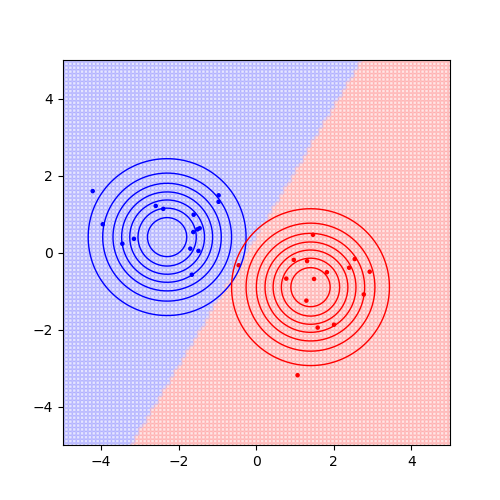
\includegraphics[scale=0.7]{img/lda.png}
    \caption{GDA of Data Generated from 2 Gaussisans centered at $(-2.3, 0.4)$ and $(1.4, -0.9)$ with unit covariance. The decision boundary is slightly off since MLE approximates the true means. }
    \label{fig:lda}
  \end{figure}

\subsection{Quadratic Discriminant Analysis} 

  Now let's do the general form. 

  \begin{definition}[Gaussian Discriminant Analysis] 
    The \textbf{GDA model} is a generative binary classification model that assumes the data is generated as 
    \begin{align} 
      y & \sim \text{Bernoulli}(\pi) \\
      x \mid y = 0 & \sim \mathcal{N} (\mu_0, \Sigma_0) \\
      x \mid y = 1 & \sim \mathcal{N} (\mu_1, \Sigma_1)
    \end{align}
    where the parameters are $\theta = \{\pi, \mu_0, \mu_1, \Sigma_0, \Sigma_1\}$. This results in 
    \begin{equation}
      f(x) = \begin{cases} 
        0 & \text{ if } p(x \mid y = 0) \geq p(x \mid y = 1) \\  
        1 & \text{ if else}
      \end{cases}
    \end{equation}
  \end{definition} 

  \begin{theorem}[Maximum Likelihood Estimate]
    
  \end{theorem}

  We can simplify the computation to the thresholding.  

  \begin{theorem}
    If $X \mid Y = 0 \sim N(\mu_0, \Sigma_0)$ and $X \mid Y = 1 \sim N(\mu_1, \Sigma_1)$, then the Bayes rule is
    \begin{equation}
      f^{\ast}(x) = \begin{cases}
        1 & \text{if } r_1^2 < r_0^2 + 2\log\left(\frac{\pi_1}{1-\pi_1}\right) + \log\left(\frac{|\Sigma_0|}{|\Sigma_1|}\right) \\
        0 & \text{otherwise}
      \end{cases}
    \end{equation}
    where $r_i^2 = (x - \mu_i)^T \Sigma_i^{-1} (x - \mu_i)$ for $i = 1, 2$ is the Mahalanobis distance.
  \end{theorem}
  \begin{proof}
    By definition, the Bayes rule is $h^{\ast}(x) = I(\pi_1 p_1(x) > (1 - \pi_1)p_0(x))$. Plug-in the specific forms of $p_0$ and $p_1$ and take the logarithms we get $h^{\ast}(x) = 1$ if and only if
    \begin{align}
      &(x - \mu_1)^T \Sigma_1^{-1} (x - \mu_1) - 2\log\pi_1 + \log(|\Sigma_1|) \\
      &\quad < (x - \mu_0)^T \Sigma_0^{-1} (x - \mu_0) - 2\log(1 - \pi_1) + \log(|\Sigma_0|).
    \end{align}
    
    The theorem immediately follows from some simple algebra.
  \end{proof} 

  \begin{theorem}[Decision Boundary is Quadratic]
    
  \end{theorem}
  \begin{proof}
    
  \end{proof}

\subsection{Multiclass GDA} 

  \begin{theorem}
    Let $R(f) = \mathbb{P}(f(X) \neq Y)$ be the classification error of a classification rule $f(x)$. The Bayes rule $f^{\ast}(X)$ minimizing $R(f)$ can be written as
    \begin{equation}
      f^{\ast}(x) = \argmax_k \mathbb{P}(Y = k \mid X = x)
    \end{equation}
  \end{theorem}
  \begin{proof}
    We have
    \begin{align}
      R(f) &= 1 - \mathbb{P}(f(X) = Y) \\
      &= 1 - \sum_{k=0}^{K-1} \mathbb{P}(f(X) = k, Y = k) \\
      &= 1 - \sum_{k=0}^{K-1} \mathbb{E}\left[I(f(X) = k)\mathbb{P}(Y = k \mid X)\right]
    \end{align}
    
    It's clear that $f^{\ast}(X) = \argmax_k \mathbb{P}(Y = k \mid X)$ achieves the minimized classification error $1 - \mathbb{E}[\max_k \mathbb{P}(Y = k \mid X)]$.
  \end{proof}

  Let $\pi_k = \mathbb{P}(Y = k)$. The next theorem extends QDA and LDA to the multiclass setting.

  \begin{theorem}
    Suppose that $Y \in \{0, \ldots, K - 1\}$ with $K \geq 2$. If $p_k(x) = p(x \mid Y = k)$ is Gaussian: $X \mid Y = k \sim N(\mu_k, \Sigma_k)$, the Bayes rule for the multiclass QDA can be written as
    \begin{equation}
      f^{\ast}(x) = \argmax_k \delta_k(x)
    \end{equation}
    where
    \begin{equation}
      \delta_k(x) = -\frac{1}{2}\log|\Sigma_k| - \frac{1}{2}(x - \mu_k)^T\Sigma_k^{-1}(x - \mu_k) + \log\pi_k.
    \end{equation}
    If all Gaussians have an equal variance $\Sigma$, then
    \begin{equation}
      \delta_k(x) = x^T\Sigma^{-1}\mu_k - \frac{1}{2}\mu_k^T\Sigma^{-1}\mu_k + \log\pi_k.
    \end{equation}
  \end{theorem}

  Let $n_k = \sum_i \mathbbm{1}(y_i = k)$ for $k = 0, \ldots, K - 1$. The estimated sample quantities of $\pi_k$, $\mu_k$, $\Sigma_k$, and $\Sigma$ are:
  \begin{align}
    \hat{\pi}_k &= \frac{1}{n}\sum_{i=1}^n \mathbbm{1}(y_i = k), \quad \hat{\mu}_k = \frac{1}{n_k}\sum_{i: Y_i = k} X_i, \\
    \hat{\Sigma}_k &= \frac{1}{n_k - 1}\sum_{i: Y_i = k} (X_i - \hat{\mu}_k)(X_i - \hat{\mu}_k)^T, \\
    \hat{\Sigma} &= \frac{\sum_{k=0}^{K-1}(n_k - 1)\hat{\Sigma}_k}{n - K}.
  \end{align}


